\section{Introduction}

The notion of a balanced tensor product was first given in
\cite{etingof/fusion-cat-and-homotopy}, and mainly developed mainly in
\cite{douglas/balanced-product}. It has different interpretations in various
fields:
\begin{itemize}
  \item In the theory of topological phases, this construction corresponds to
        fusing two domains (labeled by module categories) along the domain
        wall (labeled by tensor categories) \cite{kong/topological-order}.
  \item In the theory of extended topological quantum field theory, it is the
        $1$-categorical structure of a common target $3$-category $TC$
        \cite{douglas/dualizable-tensor-categories}.
  \item In the theory of vertex operator algebras (VOA), this construction helps
        classify the full bulk CFTs (as explained in
        \cite{gannon/exotic-quantum-subgroup}), and constructing new VOAs
        \cite{gannon/sln-II}.
  \item In the theory of tensor categories itself, it closely relates to the
        categorical center construction. In particular, the Drinfeld center
        $Z(C)$ of $C$ is equivalent to $C \boxtimes_{C \boxtimes C^{op}} C$
        \cite{kirillov/string-net-tv}
        \cite{douglas/dualizable-tensor-categories}.
\end{itemize}

Before this work, several algebraic constructions for balanced tensor products
were known, including categories of modules \cite{douglas/balanced-product},
internal Hom spaces \cite{davydov/picard}, and generalized categorical centers
\cite{etingof/fusion-cat-and-homotopy} \cite{kirillov/fact-homo-4d-tqft}
\cite{hoek/master}. These approaches well-captured the algebraic aspects of
balanced tensor products.

In this paper, we provide a topological construction based on skein theory,
which strikes a better mix between algebra and topology. This approach has at
least two advantages over previous constructions.

\subsection{Advantages}

\begin{enumerate}
  \item Its topological nature serves as the crucial element in demonstrating
        the necessity of skeins in Lurie's fully extended field theories in
        dimension $3$ \cite{lurie/tqft}. %I dont understand the reference to Lurie and skeins%
  \item It generalizes seamlessly to balanced tensor products involving more
        than two module categories, as shown by the following expression:
        \[ {}_{A}{M}_{B} \boxtimes_{B} {}_{B}{N}_{C} \boxtimes_{{C}} {}_{C}{L}_{D} \ldots \] %in the other models you can also do repeated products%
\end{enumerate}

\subsection{Applications} \label{section/applications}

\begin{enumerate}
  \item \textbf{(Skein Nature of eTFTs)} In an upcoming work
        \cite{guu/tv-as-3-functor}, we build on the main result presented here
        to prove the long-anticipated theorem that the Turaev-Viro state sum
        model \cite{viro/turaev-viro-model} naturally and necessarily emerges
        from the 3-functor in the classification of fully extended field
        theories \cite{lurie/tqft}. %here cite dualizable tensor categories paper%
  \item \textbf{(No-Go: Detection of Exotic Smooth Structures)} We anticipate
        that this approach can be extended to its 4D analogue, the
        Crane-Yetter model. Additionally, this strategy should apply to a
        broader generalization based on fusion 2-categories, as explored in
        \cite{douglas/fusion-2-cat-4d-tqft}. Proving this would lend support
        to the conjecture proposed there, which suggests that despite the
        construction's generality and power, it remains an extended
        topological field theory and therefore cannot detect exotic structures
        \cite{reutter/no-go-exotic}.
  \item \textbf{(Factorization Homology)} The main result of this paper
        provides a simple reproof of the result in
        \cite{kirillov/fact-homo-4d-tqft} that shows equivalence between the
        Crane-Yetter model and factorization homology
        \cite{ayala/factorization-homology} in $4$D (the excision property).
  \item \textbf{(Defected TFTs)} We expect work being useful in the study of
        defect field theories, such as in \cite{meusburger/defect-tv}.
  \item \textbf{(Computations in Tensor / Higher Categories)} Given that the
        Drinfeld center is a specific instance of the balanced tensor product,
        we expect this paper will contribute to recent advancements,
        particularly the explicit computation of centers as explored in
        \cite{maurer/computing-center}, and further develop the computational
        aspects of balanced tensor products.
\end{enumerate}

\subsection{Conventions}\label{subsection/conventions}

For simplicity, throughout the whole paper, unless otherwise mentioned, we assume the following.
\begin{enumerate}
  \item The base field is $\mathbb{C}$, the field of complex numbers.
  \item Every tensor category is finite, semisimple, pivotal, and defined over $\mathbb{C}$. %why pivotal?%
  \item Every (bi-)module category is finite, semisimple, and defined over
  $\mathbb{C}$. %we already said everything is over C%
  \item Every (bi-)module category functor is right exact (following
        \cite{douglas/balanced-product}).
        % TODO Why do we need right-exactness? Does this mean we have to check
        % right-exactness for our result as well?
        % ANSWER: Every functor M\to N is automatically both left and right exact when M is semisimple.
\end{enumerate}

\subsection{A Note to Experts}\label{subsection/a-note-to-experts}

The main theorem provides an algebraic model for balanced tensor products with
mathematical rigor, utilizing the skein construction. We do not claim to
introduce novel ideas here: This approach closely mirrors the domain-wall
perspective in topological phase theory, as outlined in
\cite{kong/topological-order}. In fact, the essential techniques have been
used in many places to study the Drinfeld center
$Z(C) \simeq C \boxtimes_{CC} C$ (e.g. \cite{kirillov/string-net-tv}). This
work is merely a generalization of it to the context of field theories with
defects.

In this work, we assume ideal conditions—finiteness, semisimplicity, and
pivotality (see \ref{subsection/conventions}). While it is both possible and
beneficial to relax some of these assumptions, for simplicity, we leave such
generalizations for future work. For example, we expect our proof works even
if pivotality is demoted to rigidity.

\section{Balanced Tensor Product (Algebra)}\label{section/balanced-tensor-product}

\noindent In this section we recall the definition of the balanced tensor product
from \cite{douglas/balanced-product}.

\begin{definition} (Balanced Module Category Functor)

  \noindent Let $C, D, E$ be tensor categories. Let $_{C}M_{D}$ be a
  $C{\text -}D$ bimodule category, $_{D}N_{E}$ be a $D{\text -}E$ bimodule
  category, $_{C}L_{E}$ be a $C{\text -}E$ bimodule category. \quad Then a
  $D$-balanced $C{\text -}E$ bimodule category functor $M \times N\to L$
  is a pair
  \[(M \times N \xrightarrow{F} L, \alpha)\] where $F$ is a bilinear $C{\text -}E$
  bimodule category functor and $\alpha$ is a natural isomorphism between the
  following two functors from $M \times D \times N$ to $L$
  \[
    \begin{tikzcd}
      M \times D \times N \arrow[r] \arrow[dr] &
      M \times N \arrow[d, Rightarrow, "\alpha"] \arrow[r, "F"] &
      L \\
      & M \times N \arrow[ur, "F"'] \\
    \end{tikzcd}
  \]
  where the object $(m,d,n)$ in $M \times D \times N$ is sent by the first
  upper arrow to $(m \lhd d, n)$, and by the first lower arrow to $(m, d \rhd n)$.
\end{definition}

% TODO
% \begin{remark}
%   The triangle and pentagonal identities for $D$ is automatically satisfied
%   [TODO: see Jin's note 20240906-110000 p.2].
% \end{remark}

\begin{definition} (Balanced Natural Transformation)

  \noindent Let $C, D, E$ be tensor categories. Let $_{C}M_{D}$ be a $C{\text -}D$
  bimodule category, $_{D}N_{E}$ be a $D{\text -}E$ bimodule category, $_{C}L_{E}$ be
  a $C{\text -}E$ bimodule category. Let $F, F'$ be $D$-balanced $C{\text -}E$ bimodule
  category functors from $M \times N$ to $L$. A $D$-balanced transformation
  from $F$ to $F'$ is a natural transformation $ F \xrightarrow{\eta} F'$ such
  that the following diagram commutes (in a naturally compatible way with the
  $C{\text -}E$ bimodule structures.)

  \[
    \begin{tikzcd}
      F(m \lhd c, n) \arrow[r, "\alpha_{m,c,n}"] \arrow[d, "\eta_{m \lhd c, n}"'] &
      F(m, c \rhd n) \arrow[d, "\eta_{m, c \rhd n}"] \\
      F'(m \lhd c, n) \arrow[r, "\alpha_{m,c,n}'"'] &
      F'(m, c \rhd n)
    \end{tikzcd}
  \]
\end{definition}

\begin{definition} (Category of Balanced Functors)

  \noindent Let $C, D, E$ be tensor categories. Let $_{C}M_{D}$ be a
  $C{\text -}D$ bimodule category, $_{D}N_{E}$ be a $D{\text -}E$ bimodule
  category, $_{C}L_{E}$ be a $C{\text -}E$ bimodule category. Let $F, F'$ be
  $D$-balanced $C{\text -}E$ bimodule category functors from $M \times N$ to $L$.
  \quad Then the category of balanced functors
  $Fun^{D{\text -}bal}_{C,E}(M \times N, L)$ is defined to be the category whose
  objects are $D$-balanced $C{\text -}E$ bimodule category functors
  $M \times N \to L$ and whose morphisms are $D$-balanced natural transformations.
\end{definition}

% TODO: In this definition, I need M, N are semisimple already. But add
% a later remark saying that this can be circumvented.

\begin{definition} (Balanced Tensor Product)

  \noindent Let $C, D, E$ be tensor categories. Let $_{C}M_{D}$ be a
  $C{\text -}D$ bimodule category, and $_{D}N_{E}$ be a $D{\text -}E$ bimodule
  category. \quad Then the balanced tensor product $_{C}(M \boxtimes_{D} N)_{E}$ is
  the $C{\text -}E$ bimodule category defined as the initial $D$-balanced
  module functor from $M \times N$; i.e. for each map from $M \times N$ to some
  $C{\text -}E$ bimodule category $L$, there exists a unique $C{\text -}E$
  bimodule category functor $G$ such that the following diagram commutes,

  \[
    \begin{tikzcd}
      M \times N \arrow[r, "F"] \arrow[d, "\boxtimes_{D}"'] & L \\
      _{C}(M \boxtimes_{D} N)_{E} \arrow[ur, "G"']
    \end{tikzcd}
  \]

  \noindent and that it induces an equivalence of categories
  \[Fun_{C,E}(M \boxtimes_{D} N, L) \simeq Fun_{C,E}^{D{\text -}bal}(M \times N, L).\]
\end{definition}

\begin{definition} (Balanced Tensor Product)

  \noindent Let $C, D, E$ be tensor categories. Let $_{C}M_{D}$ be a
  $C{\text -}D$ bimodule category, and $_{D}N_{E}$ be a $D{\text -}E$ bimodule
  category. \quad Then a balanced tensor product of $M$ with $N$ over $D$ is
  a $C{\text -}E$ bimodule category $_{C}(M \boxtimes_{D} N)_{E}$ equipped with a $D$-balanced $C{\text -}E$ bimodule functor $M\times N\to _{C}(M \boxtimes_{D} N)_{E}$ such that the induced map \[Fun_{C,E}(M \boxtimes_{D} N, L) \to Fun_{C,E}^{D{\text -}bal}(M \times N, L)\] is an equivalence of categories. \end{definition}


\section{Skein Construction (Topology)}\label{section/skein-construction}

\begin{definition} (Pre-Skein Category)

  \noindent Let $C$ be a tensor category. Let $M_{C}$ and $ _{C}N$ be module
  categories. \quad Define the pre-skein category $p.sk(M,C,N)$ to be the
  category $P$ with $Obj(P) = Obj(M \boxtimes N)$, and the morphism spaces
  $Mor_{P}((m \boxtimes n), (m' \boxtimes n'))$ are defined to be the vector space
  $(V \,/ \sim)$, where
  \[
    V := \oplus_{c,\overline{c} \in Obj(C)} Hom_{M}(m, m' \lhd c) \otimes Hom_{C}(c,\overline{c}) \otimes Hom_{N} (\overline{c} \rhd n, n'),
  \]
  and the relations $\sim$ are generated by the following types of relations
  \begin{align}
    \phi \otimes (\overline{\pi} \circ \pi) \otimes \psi &- (\phi_{\pi} \otimes \overline{\pi} \otimes \psi) \label{relation/a} \\
    \phi \otimes (\overline{\pi} \circ \pi) \otimes \psi &- (\phi \otimes \pi \otimes {}_{\overline{\pi}}\psi) \label{relation/b},
  \end{align}
  where
  \begin{align}
    \phi_{\pi}  &:= \left( m \xrightarrow{\phi} m' \lhd c \xrightarrow{1_{m'} \lhd \pi} m' \lhd c' \right)\\
    {}_{\overline{\pi}}\psi &:= \left( \overline{c} \rhd n \xrightarrow{\overline{\pi} \rhd 1_{n}} \overline{\overline{c}} \rhd n \xrightarrow{\psi} n' \right)
  \end{align}

  % % TODO: Make a better picture.
  % \begin{center}
  %   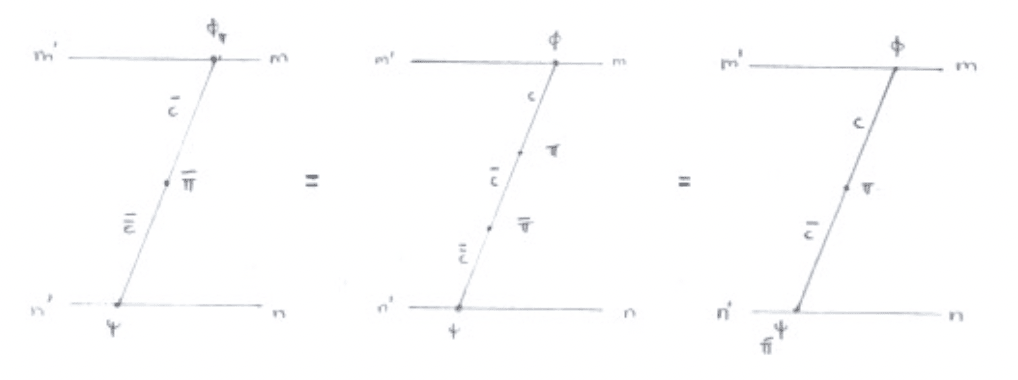
\includegraphics[width=18cm]{1}
  % \end{center}
  \begin{center}
    \includesvg[width=18cm]{drawing-1}
  \end{center}

  \noindent We define the composition on the level of $V$. It is
  straightforward to check that it descends properly to $(V \, / \sim)$ using
  the $2$-categorically compositional nature of tensor categories.
  % TODO: If have time, add a complete proof for this claim, perhaps in the appendix.
  The composition
  \[
    (\phi' \otimes \pi' \otimes \psi' ) \circ (\phi \otimes \pi \otimes \psi)
  \]
  is defined to be $(\phi'' \otimes \pi'' \otimes \psi'')$ where
  \begin{itemize}
    \item
    $\pi'' \in Hom_{C}(c' \otimes c, \overline{c}' \otimes \overline{c})$ is equal to
    \[
      c' \otimes c \xrightarrow{\pi' \otimes \pi} \overline{c'} \otimes \overline{c},
    \]
    \item
    \noindent $\phi'' \in Hom_{M}(m, m'' \lhd (c' \otimes c))$ is equal to
    \[
      m \xrightarrow{\phi} m' \lhd c \xrightarrow{\phi' \lhd 1_{c}} (m'' \lhd c') \lhd c \xrightarrow[\sim]{\alpha} m'' \lhd (c' \otimes c),
    \]
    \item
    \noindent $\psi'' \in Hom_{N}((\overline{c}' \otimes \overline{c}) \rhd n, n'')$ is equal to
    \[
      (\overline{c}' \otimes \overline{c}) \rhd n \xrightarrow[\sim]{\alpha} \overline{c}' \rhd (\overline{c} \rhd n) \xrightarrow{1_{\overline{c}'} \rhd \psi} \overline{c}' \rhd n' \xrightarrow{\psi'} n''.
    \]
  \end{itemize}

  % % TODO: Make a better picture.
  % \begin{center}
  %   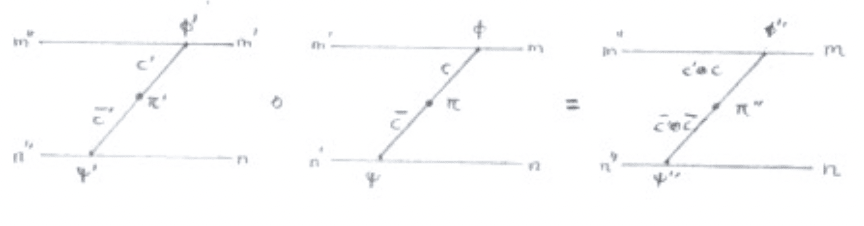
\includegraphics[width=18cm]{2}
  % \end{center}
  \begin{center}
    \includesvg[width=18cm]{drawing-2}
  \end{center}

  \noindent Finally, extend the definition of the morphism spaces to those between
  general objects via direct sum.

\end{definition}

\begin{notation} (${}^{m'}_{n'}I^{m}_{n}$)

  \noindent Denote the equivalence class of the vector
  $(\phi \otimes \pi \otimes \psi) \in V$ by
  \[\III{m'}{n'}{m}{n}{\phi}{\psi}{c}{\pi}{c'}.\]
  When $m' = m$ and $n' = n$, we omit the primed symbols and write
  \[
    \III{}{}{m}{n}{\phi}{\psi}{c}{\pi}{c'} :=
    \III{m}{n}{m}{n}{\phi}{\psi}{c}{\pi}{c'}.
  \]
  When $\pi = 1_{c}$ (thus $c' = c$), we abbreviate it further to
  \[
    \II{m'}{n'}{m}{n}{\phi}{\psi}{c} :=
    \III{m'}{n'}{m}{n}{\phi}{\psi}{c}{1_{c}}{c},
  \]
  and
  \[
    \II{}{}{m}{n}{\phi}{\psi}{c} :=
    \III{m}{n}{m}{n}{\phi}{\psi}{c}{1_{c}}{c}.
  \]
\end{notation}

\begin{remark}\label{remark/skein-nature-of-the-notation-I} (Skein Nature of the Notation ${}^{m'}_{n'}I^{m}_{n}$)

  \noindent Informally yet instructively, it is helpful to view
  $\III{m'}{n'}{m}{n}{\phi}{\psi}{c}{\pi}{c'}$ as a skein flowing from the right to
  the left, starting from $m \boxtimes n$ to $m' \boxtimes n'$, passing through $\phi \boxtimes \psi$;
  during the process, the upper strain emits a particle $c$ at $\phi$, which
  transforms to via $\pi$ to $\overline{c}$, and hits the lower strain at
  $\psi$. Hence under the defined composition rule (see the equation for
  $\phi'' \otimes \pi'' \otimes \psi''$ above), we have
  \[
    \III{m''}{n''}{m'}{n'}{\phi'}{\psi'}{c'}{\pi'}{\overline{c}'} \circ
    \III{m'}{n'}{m}{n}{\phi}{\psi}{c}{\pi}{\overline{c}} =
    \III{m''}{n''}{m}{n}{\phi''}{\psi'}{c' \otimes c}{\pi''}{\overline{c}' \otimes \overline{c}}.
  \]
\end{remark}

\begin{remark}\label{remark/hom-space-reduction} (Hom Space Reduction)

  \noindent By the relations in the definition, the transformation
  \[
    \pi = 1_{\overline{c}} \circ \pi = \pi \circ 1_{c}
  \]
  can be absorbed into each of the strain, so
  \[
    \II{m'}{n'}{m}{n}{\phi}{{}_{\pi}\psi}{c} =
    \III{m'}{n'}{m}{n}{\phi}{{}_{\pi}\psi}{c}{1_{c}}{c} =
    \III{m'}{n'}{m}{n}{\phi}{\psi}{c}{\pi}{c'} =
    \III{m'}{n'}{m}{n}{\phi_{\pi}}{\psi}{c'}{1_{c'}}{c'} =
    \II{m'}{n'}{m}{n}{\phi_{\pi}}{\psi}{c'}.
  \]

  \noindent Furthermore, if $c \simeq \oplus_{i=1}^{l} c_{i}$, then
  \[
    \II{m'}{n'}{m}{n}{\phi}{\psi}{c} = \II{m'}{n'}{m}{n}{\phi}{\psi}{\oplus_{i=1}^{l} c_{i}} = \sum_{j=1}^{l} \III{m'}{n'}{m}{n}{\phi_{j}}{\psi}{c_{j}}{\iota_{j}}{\oplus_{i=1}^{l} c_{i}} =
    \sum_{j=1}^{l}\II{m'}{n'}{m}{n}{\phi_{j}}{\psi_{j}}{c_{j}},
  \]
  where $\iota_{j}$ denotes the $j$-th embedding map from $c_{j}$ to
  $\oplus_{i=1}^{l}c_{i}$, and the $\phi_{j}, \psi_{j}$'s denote the $j$-th
  projection of $\phi, \psi$ respectively. In particular, when
  $c \simeq x^{\oplus l}$, the this gives a reduction from
  \[
    Hom_{M}(m, m' \rhd x^{\oplus l}) \otimes Hom_{C}(x^{\oplus l}, x^{\oplus l}) \otimes Hom_{N} (x^{\oplus l} \lhd n, n')
  \]
  to
  \[
    Hom_{M}(m, m' \rhd x) \otimes Hom_{C}(x, x) \otimes Hom_{N} (x \lhd n, n').
  \]
  It is helpful to regard the result as the ``inner product'' of $\phi$ and $\psi$.
\end{remark}

\noindent The hom vector spaces are finite dimensional. An explicit basis is
constructed in \ref{proposition/basis-theorem}.

\begin{definition} \label{definition/karoubi-completion} (Karoubi Completion)

  \noindent Let $C$ be a category. \quad The Karoubi completion $Kar(C)$ of
  $C$ is defined to be the category with
  \[
    Obj(Kar(C)) = \{(c, f) \,|\, c \in Obj(C), f \in End_{C}(c), f = f^{2}\}
  \] and
  \[
    Mor_{Kar(C)}((c,f), (c', f')) = \{\overline{f} \in Hom_{C}(c,c') \,|\, \overline{f}f = \overline{f} = f'\overline{f}\},
  \]
  with the obvious composition rule.
\end{definition}

\begin{remark} \label{remark/karoubi-retract} (Karoubi Retracts)

  \noindent It is straightforward to check that every object $(c,f)$ in
  $Kar(C)$ is a retract of the original object $c = (c, 1_{c})$. So we have
  \[
    (c, f) \xrightarrow{\iota} c = (c, 1_{c}) \xrightarrow{\pi} (c, f).
  \]
\end{remark}

\begin{definition}\label{definition/skein-category} (Skein Category)

  \noindent Let $C$ be a tensor category. Let $M_{C}$ and $_{C}N$ be module
  categories. \quad Define the skein category $sk(M,C,N)$ to the Karoubi
  completion of its pre-skein category
  \[
    sk(M,C,N) := Kar(p.sk(M,C,N)).
  \]
  \noindent Thus, a typical object of the skein category $sk(M,C,N)$ is the
  direct sum of some idempotent skeins $\II{m}{n}{m}{n}{\phi}{\psi}{c}$
  ($m \in Obj(M), n \in Obj(N)$). The skein category is obviously a linear
  category.

  More generally, for any $n \in \mathbb{N}$, let
  $C_{0}, C_{1}, \ldots, C_{n}$ be tensor categories. Let
  ${}_{C_{0}}M^{1}_{C_{1}}, \, {}_{C_{1}}M^{2}_{C_{2}}, \ldots, {}_{C_{n{\text -}1}}M^{n}_{C_{n}}$
  be bimodule categories. One can in a similar way define the
  $C_{0}{\text -}C_{n}$ bimodule category
  \[
    sk(M^{1}, C_{1}, M^{2}, C_{2}, M^{3}, \ldots, C_{n{\text -}1}, M^{n}).
  \]
  % % TODO: Make a better picture.
  % \begin{center}
  %   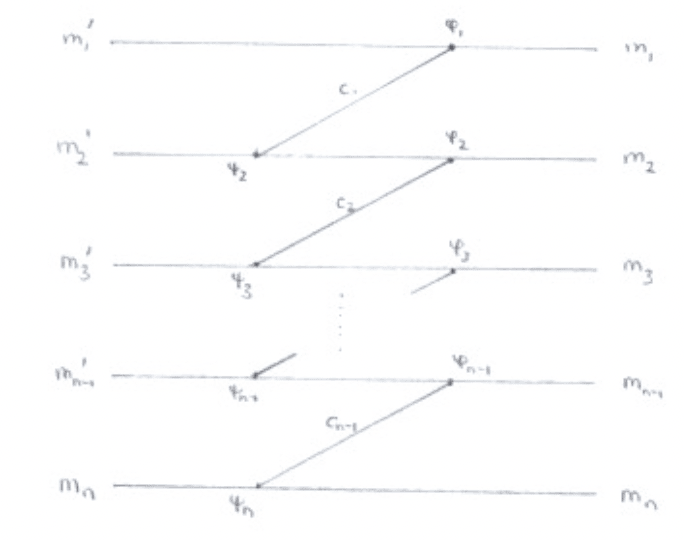
\includegraphics[width=12cm]{3}
  % \end{center}
  \begin{center}
    \includesvg[width=12cm]{drawing-3}
  \end{center}

\end{definition}

\begin{definition} \label{definition/induced-functor-on-skein-category} (Induced Functor on Skein Category)

  \noindent Assume the notation in \ref{definition/skein-category}. Let
  $1 \leq i \leq n$, and let $F: M^{i} \to M'^{i}$ be a
  $C_{i{\text -}1}{\text -}C_{i}$ bimodule category functor. \quad Then $F$
  naturally induces a linear functor between the skein categories
  \[
    sk(M^{1}, C_{1}, M^{2}, C_{2}, M^{3}, \ldots M^{i} \ldots, C_{n{\text -}1}, M^{n})
    \xrightarrow{F}
    sk(M^{1}, C_{1}, M^{2}, C_{2}, M^{3}, \ldots M'^{i} \ldots, C_{n{\text -}1}, M^{n}).
  \]
  For example, if $n=2$, $M^{1} = M$, $M^{2} = N$, $C^{1} = C$, $N \xrightarrow{F} N'$
  (with the left $C$-module structure given by $\alpha$), then we have an
  induced linear functor $sk(M,C,N) \to sk(M,C,N')$ sending the objects and morphisms via the map:
  \[
    \II{m'}{n'}{m}{n}{\phi}{\psi}{c}
    \quad \mapsto \quad
    \II{m'}{F(n')}{m}{F(n)}{\phi}{F(\psi) \circ \alpha}{c}.
  \]
\end{definition}

\noindent The main result of this paper is to show that the skein category
$sk(M,C,N)$ is equivalent to $M \boxtimes_{C} N$, and that the induced functor $M \boxtimes_{C} N \to M \boxtimes_{C} N'$
coincides with the one in \ref{definition/induced-functor-on-skein-category}
(proven in \ref{lemma/main-lemma}, \ref{theorem/main-theorem}). A necessary
ingredient is the canonical map $\boxtimes_{C}$ given in the defining universal
property.

\begin{definition}\label{definition/canonical-map} (Canonical Map $\boxtimes_{C}$)

  \noindent Let $C$ be a tensor category, and $M_{C}, _{C}N$ be module
  categories. \quad Define the functor
  \[
    M \times N \xrightarrow{\boxtimes_{C}} sk(M,C,N)
  \]
  to send the object $(m,n)$ to the object $\II{m}{n}{m}{n}{1_{m}}{1_{n}}{1_{1}}$, and the morphism
  \[
    (m,n) \xrightarrow{(\phi, \psi)} (m', n')
  \]
  to the morphism $\II{m'}{n'}{m}{n}{\phi}{\psi}{1_{1}}$.
\end{definition}

\noindent From the main theorem, we must have $sk(M,C,C) \simeq M$. To quickly
convince the reader that the main theorem is true before it is proven, we
provide another direct proof for this equivalence in the appendix (cf
\ref{proposition/degenerated-main-theorem}).

\hfill\break
\noindent We prove another lemma that will be useful later.

\begin{lemma}\label{lemma/I-provides-subobject} (Objects are Retracts)

  \noindent Let $C$ be a tensor category, and $M_{C}, _{C}N$ be module
  categories. \quad Then any typical object $\II{}{}{m}{n}{\phi}{\psi}{c}$ in
  $sk(M,C,N)$ is a retract (in particular, a subobject) of the canonical
  object $\boxtimes_{C}((m,n)) = \II{}{}{m}{n}{1_{m}}{1_{n}}{1}$.
\end{lemma}
\begin{proof}
  This directly follows from \ref{remark/karoubi-retract}.
\end{proof}

\section{Proof of the Main Equivalence Theorem}\label{section/proof-of-equivalence}

Unless specified otherwise, throughout this section, let $C, D, E$ be tensor
categories, let $M_{C}$ and $_{C}N$ be module categories, and let $L$ be a
linear category. We prove our main theorem (\ref{theorem/main-theorem}) in this section, justifying
that the skein construction $sk(M,C,N)$ is isomorphic to $M \boxtimes_{C} N$, and the
obvious generalization to the case of more bimodule categories.

\begin{lemma}\label{lemma/construction-of-theta} (Construction of $\Theta$)

  \noindent There exists a linear functor
  \[
    \Theta: Fun(sk(M,C,N), L) \to Fun^{C{\text -}bal}(M \times N, L).
  \]
\end{lemma}

\noindent We construct $\Theta$ explicitly in the proof.

\begin{proof}
  \noindent (Object) Let $G$ be an object of the domain. Define $\Theta(G)$ to
  be $F := G \circ \boxtimes_{C} \in Fun(M \times N, L)$. We shall provide the
  balanced structure $\alpha$ for $F$, so that $(F, \alpha)$ is $C$-balanced. 
  We need to provide the $C$-balanced data for $F$:
  \[
    \alpha_{m,c,n}: F(m \lhd c, n) =
    G(\II{}{}{mc}{n}{1}{1}{1})
    \xrightarrow{\sim} G(\II{}{}{m}{cn}{1}{1}{1})
    = F(m, c \rhd n),
  \]
  which is clearly satisfied by $G(\II{m}{cn}{mc}{n}{1}{1}{c}).$ So defined
  $\alpha$ is clearly natural.

  \noindent (Morphism) Let $G \xrightarrow{\eta} G'$ be a morphism in
  $Fun(sk(M,C,N), L)$. Its image under $\Theta$ is simply the horizontal
  composition $\eta \star (1_{\boxtimes_{C}})$. The remaining commutativity to be checked
  % TODO: cf p11 of Jin's note 20240906-110000
  is a direct consequence of $\eta$'s naturality.
\end{proof}

\begin{lemma}\label{lemma/theta-is-faithful} ($\Theta$ is faithful)

  \noindent The linear functor $\Theta$ (cf. \ref{lemma/construction-of-theta}) is faithful.
\end{lemma}

\begin{proof}
  (We use the same notation found in this section.) This amounts to showing
  that the following map is an injective linear map:
  \[
    (G \xrightarrow{\eta} G') \mapsto (F \xrightarrow{\Theta(\eta) = \eta \star (1_{\boxtimes_{C}})} F').
  \]
  It is clearly linear. For injectivity, we notice that whenever we have
  linear functors
  \[
    X \xrightarrow{f} Y,\quad Y \xrightarrow{g, g'} Z,
  \]
  and a linear natural transformation $\eta: g \to g'$, then the map $(\eta \mapsto \eta \star 1_{f})$ is injective is equivalent to
  \[
    (\forall x \in Obj(X), \eta_{f(x)} = 0) \Rightarrow (\forall y \in Obj(Y), \eta_{y} = 0).
  \]
  This holds if $f$ is surjective on objects. However, in our case
  $f = \boxtimes_{C}$ is not as strong. Fortunately, clearly it also holds if
  $f$ is almost-surjective, in the sense that each $y \in Obj(Y)$ has an
  $x \in Obj(X)$ such that $y$ is a retract of $f(X)$. Indeed,
  \[
    1_{g(y)} = g(1_{y}) = g(\pi_{y} \circ \iota_{y}),
  \]
  so
  \[
    (g(y) \xrightarrow{\eta_{y}} g'(y)) = \eta_{y} \circ 1_{g(y)} = \eta_{y} \circ g(\pi \circ \iota) = g(\pi) \circ \eta_{f(x)} \circ g(\iota) = g(\pi) \circ 0 \circ g(\iota) = 0.
  \]
  This applies to our case by putting $f = \boxtimes_{C}$ and $g = G$, because
  each object $\II{}{}{m}{n}{\phi}{\psi}{c}$ is clearly a retract of
  $\boxtimes_{C}(m,n) = \II{}{}{m}{n}{1}{1}{1}$. Therefore, $\Theta$ is faithful.
\end{proof}

\begin{lemma}\label{lemma/theta-is-full} ($\Theta$ is full)

  \noindent The linear functor $\Theta$ (cf. \ref{lemma/construction-of-theta}) is full.
\end{lemma}

\begin{proof}
  We need to show that for any $C$-balanced natural transformation
  \[
    \nu: G \circ \boxtimes_{C} = \Theta(G) \to \Theta(G') = G' \circ \boxtimes_{C}
  \]
  there is $\mu: G \to G'$ such that $\nu = \mu \star 1_{\boxtimes_{C}}$. The data $\nu$ are the maps
  \[
    \nu_{(m,n)}: G(\II{}{}{m}{n}{1}{1}{1}) \to G'(\II{}{}{m}{n}{1}{1}{1}).
  \]
  We only need to extend these data to all objects in $sk(M,C,N)$, i.e. define compatible maps
  \[
    \nu_{\II{}{}{m}{n}{\phi}{\psi}{c}}: G(\II{}{}{m}{n}{\phi}{\psi}{c}) \to G'(\II{}{}{m}{n}{\phi}{\psi}{c}).
  \]
  It is straightforward to check that the following works:
  \[
    \nu_{\II{}{}{m}{n}{\phi}{\psi}{c}}:= G(\II{}{}{m}{n}{\phi}{\psi}{c})
    \xrightarrow{G(\iota)}
    G(\II{}{}{m}{n}{1}{1}{1})
    \xrightarrow{\nu_{(m,n)}}
    G'(\II{}{}{m}{n}{1}{1}{1})
    \xrightarrow{G'(\pi)}
    G'(\II{}{}{m}{n}{\phi}{\psi}{c}),
  \]
  where $\iota$ and $\pi$ are the inclusion and projection (see
  Lemma \ref{lemma/I-provides-subobject}).
\end{proof}

\noindent To prove that $\Theta$ is essentially surjective, we need the following
lemma.

\begin{lemma} (Images of skeins) \label{lemma/image-of-skein}
  % TODO: Discussion: Can we relax conditions? We need to use the basis theorem,
  % so it seems that we must require semisimplicity here.

  \noindent
  Let $(F,\alpha) \in Fun^{C{\text -}bal}(M \times N, L)$. For each morphism
  in $sk(M,C,N)$ of the form $\III{m'}{n'}{m}{n}{\phi}{\psi}{c}{\pi}{c'}$,
  define the image of it under $\tilde{F}$ to be the composed morphism
  \[
    F(m,n)
    \xrightarrow{F(\phi \times 1)}
    F(m' \lhd c, n)
    \xrightarrow{F((1 \lhd \pi) \times 1)}
    F(m' \lhd c', n)
    \xrightarrow[\sim]{\alpha}
    F(m', c' \rhd n)
    \xrightarrow{F(1 \times \psi)}
    F(m',n').
  \]
  Suppose we have two skeins $\II{m'}{n'}{m}{n}{\phi}{\psi}{c}$ and
  $ \II{m'}{n'}{m}{n}{\phi'}{\psi'}{c'}$ as identical morphisms in $sk(M,C,N)$
  (recall the definitional relations (\ref{relation/a}) (\ref{relation/b})).

  \noindent Then
  \begin{equation} \label{eqn/a}
    \tilde{F}(\II{m'}{n'}{m}{n}{\phi}{\psi}{c}) = \tilde{F}(\II{m'}{n'}{m}{n}{\phi'}{\psi'}{c'}).
  \end{equation}
  Moreover, $\tilde{F}$ preserves compositions, i.e.
  \begin{equation} \label{eqn/b}
    \tilde{F}(\II{m''}{n''}{m'}{n'}{\overline{\phi}}{\overline{\psi}}{\overline{c}} \circ \II{m'}{n'}{m}{n}{\phi}{\psi}{c})
    = \tilde{F}(\II{m''}{n''}{m'}{n'}{\overline{\phi}}{\overline{\psi}}{\overline{c}})
    \circ
    \tilde{F}(\II{m'}{n'}{m}{n}{\phi}{\psi}{c}).
  \end{equation}
\end{lemma}

\begin{proof}
  To prove the first statement (\ref{eqn/a}), check the equality against the
  definitional relations (\ref{relation/a}) (\ref{relation/b}).

  \noindent To prove the second statement (\ref{eqn/b}), note that the
  left-hand-side is
  $\tilde{F}(\II{m''}{n'}{m}{n}{\overline{\phi} \otimes \phi}{\overline{\psi} \otimes \psi}{\overline{c} \otimes c}),$
  which is
  \begin{multline*}
    F(m,n)
    \xrightarrow{F(\phi \times 1)}
    F(m' \lhd c, n)
    \xrightarrow{F((\overline{\phi} \lhd 1) \times 1)} \\
    F((m'' \lhd \overline{c}) \lhd c, n)
    \xrightarrow[\sim]{}
    F((m'' \lhd (\overline{c} \otimes c)), n)
    \xrightarrow[\sim]{\alpha}
    F(m'', (\overline{c} \otimes c) \rhd n)
    \xrightarrow[\sim]{}
    F(m'', \overline{c} \rhd (c \rhd n)) \\
    \xrightarrow{F(1 \times (1 \rhd \psi))}
    F(m'', \overline{c} \rhd n')
    \xrightarrow{F(1 \times \overline{\psi})}
    F(m'',n'').
  \end{multline*}
  On the other hand, the right-hand-side is
  \begin{multline*}
    F(m,n)
    \xrightarrow{F(\phi \times 1)}
    F(m' \lhd c, n)
    \xrightarrow[\sim]{\alpha} \\
    F(m', c \rhd n)
    \xrightarrow{F(1 \times \psi)}
    F(m', n')
    \xrightarrow{F(\overline{\phi} \times 1)}
    F(m'' \rhd \overline{c}, n') \\
    \xrightarrow[\sim]{\alpha}
    F(m'', \overline{c} \lhd n')
    \xrightarrow{F(1 \times \overline{\psi})}
    F(m'',n'').
  \end{multline*}
  To prove that they are equal, we can omit their first and their last arrows. Note that the composed arrow in left-hand-side $F(m' \lhd c, n) \to F(m', \overline{c} \rhd (c \rhd n))$ is, by the naturality of $\alpha$, equal to
  \[
    F(m' \lhd c, n)
    \xrightarrow[\sim]{\alpha}
    F(m', c \rhd n)
    \xrightarrow{F(\overline{\phi} \times 1)}
    F(m'' \lhd \overline{c}, c \rhd n)
    \xrightarrow[\sim]{\alpha}
    F(m'', \overline{c} \rhd (c \rhd n)).
  \]
  Compose this with
  \[
    F(m'', \overline{c} \rhd (c \rhd n))
    \xrightarrow{F(1 \times (1 \rhd \psi))}
    F(m', \overline{c} \rhd n'),
  \]
  then we get
  \[
    F(m' \lhd c, n)
    \xrightarrow[\sim]{\alpha}
    F(m', c \rhd n)
    \xrightarrow{F(\overline{\phi} \times 1)}
    F(m'' \lhd \overline{c}, c \rhd n)
    \xrightarrow{F(1 \times \psi)}
    F(m'' \lhd \overline{c}, n'),
  \]
  which is equal to
  \[
    F(m' \lhd c, n)
    \xrightarrow[\sim]{\alpha}
    F(m', c \rhd n)
    \xrightarrow{F(\overline{\phi} \times \psi)}
    F(m'' \lhd \overline{c}, n').
  \]
  So both sides are equal.
\end{proof}

\begin{lemma}\label{lemma/theta-is-essentially-surjective} ($\Theta$ is essentially surjective)

  \noindent The linear functor $\Theta$ (cf. \ref{lemma/construction-of-theta}) is essentially surjective.
\end{lemma}

\begin{proof}
  Let $(F, \alpha) \in Fun^{C{\text -}bal}(M \times N, L)$. It suffices to construct
  $G \in Fun(sk(M,C,N), L)$ such $\Theta(G) \simeq (F,\alpha)$. Recall that $L$ is an abelian
  category (so each $L$-morphism has an image), $F: M \times N \to L$ is a linear
  functor, and that
  \[
    F(m \lhd c, n) \xrightarrow[\sim]{\alpha_{m,c,n}} F(m, c \rhd n).
  \]

  \noindent ($G$ on objects) Recall the definition and properties of
  $\tilde{F}$ in \ref{lemma/image-of-skein}. Define
  $G(\II{}{}{m}{n}{\phi}{\psi}{c})$ to be the image (in $L$) of the
  $L$-morphism $\tilde{F}(\II{}{}{m}{n}{\phi}{\psi}{c})$. In particular, the
  image is a subobject and a quotient of $F(m,n)$.

  \noindent ($G$ on morphisms) We use $\tilde{F}$ again. Let
  $\II{m'}{n'}{m}{n}{\overline{\phi}}{\overline{\psi}}{\overline{c}}$ be a morphism
  from $\II{}{}{m}{n}{\phi}{\psi}{c}$ to $\II{}{}{m'}{n'}{\phi'}{\psi'}{c'}$. Define
  $G(\II{m'}{n'}{m}{n}{\overline{\phi}}{\overline{\psi}}{\overline{c}})$ to be the
  map induced by
  \[
    \tilde{F}(\II{m'}{n'}{m}{n}{\overline{\phi}}{\overline{\psi}}{\overline{c}}): F(m,n) \to F(m',n').
  \]
  To justify this definition, we must show that
  \[
    ker(
    \tilde{F}(\II{}{}{m'}{n'}{\phi'}{\psi'}{c'})
    \circ
    \tilde{F}(\II{m'}{n'}{m}{n}{\overline{\phi}}{\overline{\psi}}{\overline{c}})
    )
    \supseteq
    ker(\tilde{F}(\II{}{}{m}{n}{\phi}{\psi}{c})).
  \]
  By lemma \ref{lemma/image-of-skein}, $\tilde{F}$ respects compositions, so
  \[
    ker(
    \tilde{F}(\II{}{}{m'}{n'}{\phi'}{\psi'}{c'})
    \circ
    \tilde{F}(\II{m'}{n'}{m}{n}{\overline{\phi}}{\overline{\psi}}{\overline{c}})
    )
    =
    ker(
    \tilde{F}(\II{}{}{m'}{n'}{\phi'}{\psi'}{c'}
    \circ
    \II{m'}{n'}{m}{n}{\overline{\phi}}{\overline{\psi}}{\overline{c}})
    ).
  \]
  Then by the definition of $sk(M,N,C)$ and Karoubi completion,
  \[
    ker(
    \tilde{F}(\II{}{}{m'}{n'}{\phi'}{\psi'}{c'}
    \circ
    \II{m'}{n'}{m}{n}{\overline{\phi}}{\overline{\psi}}{\overline{c}})
    )
    =
    ker(
    \tilde{F}(
    \II{m'}{n'}{m}{n}{\overline{\phi}}{\overline{\psi}}{\overline{c}}
    \circ
    \II{}{}{m}{n}{\phi}{\psi}{c}
    )
    ).
  \]
  The final step is completed by using the composing property of $\tilde{F}$ again and the fact that
  $ker(a \circ b) \supseteq ker(b)$.
\end{proof}

\begin{lemma} (Main Lemma) \label{lemma/main-lemma}

  \noindent The canonical map (\ref{definition/canonical-map})
  $\boxtimes_{C}$: $M \times N \to sk(M,C,N)$ satisfies the universal property
  in the definition of $M \boxtimes_{C} N$. In particular, we have an
  equivalence of categories
  \[
    sk(M,C,N) \simeq M \boxtimes_{C} N.
  \]
\end{lemma}

% % TODO: Ask Manuel to provide a proof.
% \begin{remark}
%   The whole proof can be conceptually simplified while viewed at the level of
%   arrows. Indeed, from $M \times N$ to $sk(M,C,N)$, we have a chain of
%   functors:
%   \[
%     sk(M,C,N)
%     \leftarrow
%     psk(M,C,N)
%     \leftarrow
%     M \boxtimes N
%     \leftarrow
%     M \otimes N
%     \leftarrow
%     M \times N.
%   \]
%   All we need to show is that while applying $Fun(-, L)$, we obtain a chain of
%   equivalences:
%   \[
%     Fun(sk(M,C,N), L)
%     \rightarrow
%     Fun(psk(M,C,N), L)
%     \rightarrow
%     Fun^{C{\text -}bal}(M \boxtimes N, L)
%     \rightarrow
%     Fun^{C{\text -}bal}(M \otimes N, L)
%     \rightarrow
%     Fun^{C{\text -}bal}(M \times N, L).
%   \]
% \end{remark}

\begin{proof}
  We only need to show that $sk(M,C,N)$ is a $k$-linear category (in
  particular, an abelian category, following the definition in
  \cite{douglas/balanced-product}), and that $\boxtimes_{C}$ induces an equivalence of
  categories
  \[
    Fun(sk(M,C,N), L) \xrightarrow[\sim]{\Theta} Fun^{C{\text -}bal}(M \times N, L).
  \]
  For $k$-linearity, the crux is to show that the skein category is abelian.
  We postpone the proof to the appendix \ref{semisimple}. For the second
  statement, we constructed $\Theta$ in (\ref{lemma/construction-of-theta}), proved that $\Theta$ is faithfulness in
  (\ref{lemma/theta-is-faithful}), is full in (\ref{lemma/theta-is-full}), and is essentially surjective in (\ref{lemma/theta-is-essentially-surjective}).
\end{proof}


\begin{theorem} (Main Theorem: Skein Construction of Balanced Tensor Product) \label{theorem/main-theorem}

  \noindent (1) Let ${}_{C}M_{D}, \, {}_{D}N_{E}$ be, bimodule categories.
  \quad Then the canonical map (\ref{definition/canonical-map})
  $\boxtimes_{D}$: $M \times N \to sk(M,D,N)$ satisfies the universal property
  in the definition of ${}_{C}M_{D} \boxtimes_{D} {}_{D}N_{E}$. In particular,
  we have an equivalence of $C{\text -}E$ bimodule categories.
  \[
    {}_{C}sk(M,D,N)_{E} \simeq {}_{C}M_{D} \boxtimes_{D} {}_{D}N_{E}.
  \]

  \noindent (2) More generally, for any $n \in \mathbb{N}$, let
  $C_{0}, C_{1}, \ldots, C_{n}$ be tensor categories. Let
  ${}_{C_{0}}M^{1}_{C_{1}}, \, {}_{C_{1}}M^{2}_{C_{2}}, \ldots, {}_{C_{n{\text -}1}}M^{n}_{C_{n}}, \, $
  be bimodule categories. \quad Then we have an equivalence of
  $C_{0}{\text -}C_{n}$ bimodule categories.
  \[
    {}_{C_{0}}sk(M^{1},C_{1},M^{2},C_{2}, \ldots, C_{n{\text -}1}, M^{n})_{C_{n}}
    \simeq
    {}_{C_{0}}(M^{1}
    \boxtimes_{C_{1}}
    M^{2}
    \boxtimes_{C_{2}}
    M^{3}
    \ldots
    \boxtimes_{C_{n{\text -}1}}
    M^{n})_{C_{n}}.
  \]
  \noindent (3) Moreover, in addition to the previous part, if
  $F^{i}: M^{i} \to M'^{i}$ is a $C_{i{\text -}1}{\text -}C_{i}$ bimodule category
  functor, then the naturally induced linear functor (cf.
  \ref{definition/induced-functor-on-skein-category})
  \[
    F^{i}:
    sk(M^{1}, C_{1}, M^{2}, C_{2}, M^{3}, \ldots M^{i} \ldots, C_{n{\text -}1}, M^{n})
    \to
    sk(M^{1}, C_{1}, M^{2}, C_{2}, M^{3}, \ldots M'^{i} \ldots, C_{n{\text -}1}, M^{n}),
  \]
  corresponds to the functor
  \[
    F^{i}: M^{1} \boxtimes_{C_{1}} M^{2} \boxtimes_{C_{2}} M^{3} \boxtimes_{C_{3}} \ldots M^{i} \ldots \boxtimes_{C_{n{\text -}1}} M^{n} \to M^{1} \boxtimes_{C_{1}} M^{2} \boxtimes_{C_{2}} M^{3} \boxtimes_{C_{3}} \ldots M'^{i} \ldots \boxtimes_{C_{n{\text -}1}} M^{n}.
  \]
  under the equivalence.
\end{theorem}

\begin{proof}
  The first part is proved by restricting the proof of lemma \ref{lemma/main-lemma} to $C{\text -}E$ bimodule maps.
  The second part follows directly from induction and the first part. The third part is obvious.
\end{proof}

\begin{remark} (Application on the Turaev-Viro model)

  \noindent That the induced functor on the skein category coincides with the
  algebraic one is the key for computing values of the Turaev-Viro model in
  dimensions $(1+1)$ \cite{guu/tv-as-3-functor}.
\end{remark}

% TODO This corollary is wrong. Remove it later.
%
% \begin{corollary}\label{corollary/skein-category-is-abelian} (Skein Categories are Abelian)

%   \noindent For any $n \in \mathbb{N}$, let $C_{0}, C_{1}, \ldots, C_{n}$ be
%   tensor categories. Let
%   \[
%     {}_{C_{0}}M^{1}_{C_{1}}, \, {}_{C_{1}}M^{2}_{C_{2}}, \ldots, {}_{C_{n{\text -}1}}M^{n}_{C_{n}}, \,
%   \]
%   be bimodule categories. Then the skein category (cf
%   \ref{definition/skein-category})
%   \[
%     sk(M^{1}, C_{1}, M^{2}, C_{2}, M^{3}, \ldots M^{i} \ldots, C_{n{\text -}1}, M^{n})
%   \]
%   is an abelian category.
% \end{corollary}
% \begin{proof}
%   The proof for the case $n=2$ follows from the fact that
%   $M^{1} \boxtimes_{C_{1}} M^{2} \simeq Z_{C_{1}}(M^{1} \boxtimes M^{2})$ is
%   abelian (cf \cite{kirillov/fact-homo-4d-tqft}). The rest follows from
%   induction.
% \end{proof}

\appendix
\section{Appendix}

\subsection{$sk(M,C,N)$ is $k$-linear}

\noindent We will now prove the technical condition that the skein
category $sk(M,C,N)$ is $k$-linear in \ref{semisimple}. In particular, it is
abelian. This result completes the proof of the main lemma \ref{lemma/main-lemma}. 

From now on, we fix a field $k$.

\begin{definition}
  Denote by $\Vect_k$ the category of $k$-vector spaces. We assume all
  categories, functors and natural transformations are enriched over
  $\Vect_k$. We always write $\otimes$ instead of $\otimes_k$.
\end{definition}

\subsubsection{The construction and universal property of $sk(M,C,N)$}

Starting from a rigid monoidal category $C$ and module
categories $M_C$, $_{C}N$ we construct a Cauchy complete category $sk(M,C,N)$
with a $C$-balanced functor $M\otimes N\to sk(M,C,N)$ satisfying a certain
universal property.

\begin{definition}
  Given categories $M, N$ we define $M\otimes N$ to be the category whose
  objects are pairs $(m,n)$ with $m\in M$ and $n\in N$ and where
  $Hom_{M\otimes N}((m,n),(m',n'))=Hom_{M}(m,m')\otimes Hom_N(n,n')$.
\end{definition}

\begin{definition}
  For $C$ a monoidal category and $M_C$, $_{C}N$ module categories, we define
  a new category $M\otimes_C N$ as follows. Its objects are pairs $(m,n)$ with
  $m\in M$ and $n\in N$. The $k$-vector space
  $Hom_{M\otimes_C N}((m,n),(m',n'))$ is the quotient
  of $$\bigoplus_{c,\overline{c} \in Obj(C)} Hom_{M}(m, m' \lhd c) \otimes Hom_{C}(c,\overline{c}) \otimes Hom_{N} (\overline{c} \rhd n, n')$$
  by the subspace spanned by
  \begin{align}
    \phi \otimes (\overline{\pi} \circ \pi) \otimes \psi &- (\phi_{\pi} \otimes \overline{\pi} \otimes \psi) \label{relation/a} \\
    \phi \otimes (\overline{\pi} \circ \pi) \otimes \psi &- (\phi \otimes \pi \otimes {}_{\overline{\pi}}\psi) \label{relation/b},
  \end{align}
  where
  \begin{align}
    \phi_{\pi}  &:= \left( m \xrightarrow{\phi} m' \lhd c \xrightarrow{1_{m'} \lhd \pi} m' \lhd c' \right) \\
    {}_{\overline{\pi}}\psi &:= \left( \overline{c} \rhd n \xrightarrow{\overline{\pi} \rhd 1_{n}} \overline{\overline{c}} \rhd n \xrightarrow{\psi} n' \right)
  \end{align}
  The composition
  \[
    (\phi' \otimes \pi' \otimes \psi' ) \circ (\phi \otimes \pi \otimes \psi)
  \]
  is defined to be $(\phi'' \otimes \pi'' \otimes \psi'')$ where
  \begin{itemize}
    \item
    $\pi'' \in Hom_{C}(c' \otimes c, \overline{c}' \otimes \overline{c})$ is equal to
    \[
      c' \otimes c \xrightarrow{\pi' \otimes \pi} \overline{c'} \otimes \overline{c},
    \]
    \item
    \noindent $\phi'' \in Hom_{M}(m, m'' \lhd (c' \otimes c))$ is equal to
    \[
      m \xrightarrow{\phi} m' \lhd c \xrightarrow{\phi' \lhd 1_{c}} (m'' \lhd c') \lhd c \xrightarrow[\sim]{\alpha} m'' \lhd (c' \otimes c),
    \]
    \item
    \noindent $\psi'' \in Hom_{N}((\overline{c}' \otimes \overline{c}) \rhd n, n'')$ is equal to
    \[
      (\overline{c}' \otimes \overline{c}) \rhd n \xrightarrow[\sim]{\alpha} \overline{c}' \rhd (\overline{c} \rhd n) \xrightarrow{1_{\overline{c}'} \rhd \psi} \overline{c}' \rhd n' \xrightarrow{\psi'} n''.
    \]
  \end{itemize}
\end{definition}

\begin{remark}\label{absorb}
  We abuse notation by writing $(\phi\otimes\pi\otimes\psi)$ to denote the
  corresponding equivalence class in $Hom_{M\otimes_C N}((m,n),(m',n'))$.
  Using the defining relations, we see
  that
  \[
    (\phi\otimes\pi\otimes\psi) =
    (\phi_{\pi}\otimes\id_{\bar{c}}\otimes\psi) =
    (\phi\otimes\id_c\otimes{_{\pi}\psi}).
  \]
\end{remark}

\begin{lemma}\label{decompose}

  Any morphism in $M\otimes_C N$ can be written as a sum of composites of
  morphisms of the form $\phi\otimes\id_{1}\otimes\psi:(m,n)\to(m',n')$ and
  $\id_{m\lhd c}\otimes\id_c\otimes\id_{c\rhd n}:(m\lhd c,n)\to(m,c\rhd n).$
\end{lemma}

\begin{proof}
  First, any morphism is a sum of morphisms of the form
  $\phi\otimes\pi\otimes\psi$. By Remark \ref{absorb}, we can take
  $\pi=\id_c$. Now
  $(\phi\otimes\id_c\otimes\psi)
  =
  (\id_{m'}\otimes\id_1\otimes\psi)
  \circ
  (\id_{m'\lhd c}\otimes\id_c\otimes\id_{c\rhd n})
  \circ
  (\phi\otimes\id_1\otimes\id_n)$.
\end{proof}

\begin{definition}
  We define a functor $M\otimes N\to M\otimes_C N$ by the identity on objects
  and $\phi\otimes\psi\mapsto\phi\otimes\id_1\otimes\psi$ on morphisms. We
  define also morphisms $\beta_{m,c,n}:(m\lhd c,n)\to (m, c \rhd n)$ by
  $\beta_{m,c,n}=\id_{m\lhd c}\otimes\id_c\otimes\id_{c\lhd n}.$
\end{definition}

\begin{lemma}
  The collection of morphisms $\beta_{m,c,n}$ defines a natural transformation
  of functors $M\otimes C \otimes N\to M\otimes_C N$.
\end{lemma}

\begin{proof}
  Given $\phi:m\to m'$, $\psi: n\to n'$ and $\pi:c\to \bar{c}$ we must check
  that the following diagram commutes.
  \[
    \begin{tikzcd}
      {(m\lhd c, n)} & {(m,c\rhd n)} \\
      {(m'\lhd \bar{c}, n')} & {(m',\bar{c}\rhd n')}
      \arrow["{\beta_{m,c,n}}", from=1-1, to=1-2]
      \arrow["{(\phi\lhd\pi)\otimes\id_1\otimes\psi}"', from=1-1, to=2-1]
      \arrow["{\phi\otimes\id_1\otimes(\pi\rhd\psi)}", from=1-2, to=2-2]
      \arrow["{\beta_{m',\bar{c},n'}}"', from=2-1, to=2-2]
    \end{tikzcd}
  \]
  Using the definition of composition and the relations in the definition of
  $Hom_{M\otimes_C N}$ one can check that both composites equal
  $(\phi\lhd\id_c)\otimes\pi\otimes(\id_{\bar{c}}\rhd\psi)$.
\end{proof}

\begin{lemma}\label{balanced}
  If every object in $C$ has a right dual, then the natural transformation
  $\beta$ described above is an isomorphism, so it provides a balancing for
  the functor $M\otimes N\to M\otimes_C N$.
\end{lemma}

\begin{proof}
  Given $(m,c,n)$ we provide an explicit inverse for $\beta_{m,c,n}$. Let
  $(c^*,\eta,\epsilon)$ denote a right dual for $c$. We define
  $\beta^{-1}_{m,c,n}=(\id_m\lhd\eta)\otimes\id_{c^*}\otimes (\epsilon\rhd\id_n)$.
  To prove that this is inverse to $\beta_{m,c,n}$ we use only one of the
  snake equations.
\end{proof}

From now on, we assume that $C$ has right duals. The following universal
property characterizes $M\otimes N \to M\otimes_C N$.

\begin{proposition}\label{univ_bal}
  Let $L$ be a category and suppose $C$ has right duals. Then composition with
  $M\otimes N \to M\otimes_C N$ induces an equivalence of categories
  $Fun(M\otimes_C N,L)\to Fun^{C-bal}(M\otimes N,L)$.
\end{proposition}
\begin{proof}
The proof consists of Lemmas \ref{surjective}, \ref{faithful} and \ref{full}.  \end{proof}

\begin{lemma}\label{surjective}
  $Fun(M\otimes_C N,L)\to Fun^{C-bal}(M\otimes N,L)$ is surjective on
  objects.
\end{lemma}

\begin{proof}
  Given a $C$-balanced functor $F:M\otimes N \to L$ with balancing $\beta$, we
  must define $\tilde{F}:M\otimes_C N \to L$ such that its composite with
  $M\otimes N\to M\otimes_C N$ is $F$. We must take $\tilde{F}=F$ on objects.
  To define $\tilde{F}$ on morphisms, let $\phi\in Hom_M(m,m'\lhd c)$,
  $\pi\in Hom_C(c,\bar{c})$ and $\psi\in Hom_N(\bar{c}\rhd n,n')$. We define
  $\tilde{F}(\phi\otimes\pi\otimes\psi)$ to be the composite
  \[
    \begin{tikzcd}
      {(m,n)} & {(m'\lhd c,n)} & {(m'\lhd \bar{c},n)} & {(m',\bar{c}\rhd n)} & {(m',n')}
      \arrow["{F(\phi,n)}", from=1-1, to=1-2]
      \arrow["{F(m'\lhd\pi,n)}", from=1-2, to=1-3]
      \arrow["{\beta_{m',\bar{c},n}}", from=1-3, to=1-4]
      \arrow["{F(m',\psi)}", from=1-4, to=1-5]
    \end{tikzcd}.
  \]
  The naturality of $\beta$ with respect to morphisms in $C$ implies that this
  is equal to the composite
  \[
    \begin{tikzcd}
      {(m,n)} & {(m'\lhd c,n)} & {(m', c\rhd n)} & {(m',\bar{c}\rhd n)} & {(m',n')}
      \arrow["{F(\phi,n)}", from=1-1, to=1-2]
      \arrow["{\beta_{m',c,n}}", from=1-2, to=1-3]
      \arrow["{F(m',\pi\rhd n)}", from=1-3, to=1-4]
      \arrow["{F(m',\psi)}", from=1-4, to=1-5]
    \end{tikzcd}.
  \]
  From these two expressions it is clear that this respects the relations in
  the definition of $Hom_{M\otimes_C N}$. The proof that this respects
  composition is a straightforward calculation, using the naturality of
  $\beta$ with respect to morphisms in $M$ and $N$.
  \end{proof}

  \begin{remark}
    Using Lemma \ref{decompose}, the functor $\tilde{F}:M\otimes_C N\to L$
    whose composite with $M\otimes N\to M\otimes_C N$ is the $C$-balanced
    functor $F:M\otimes N\to L$ with balancing $\beta$ is also determined by
    $\tilde{F}(m,n)=F(m,n)$,
    $\tilde{F}(\phi\otimes\id_1\otimes\psi)=F(\phi,\psi)$ and
    $\tilde{F}(\id_{m\lhd c}\otimes\id_c\otimes\id_{c\rhd n})=\beta_{m,c,n}.$
  \end{remark}

\begin{lemma}\label{faithful}
  $Fun(M\otimes_C N,L)\to Fun^{C-bal}(M\otimes N,L)$ is faithful.
\end{lemma}

\begin{proof}
  This is immediate from the fact that $M\otimes N \to M\otimes_C N$ is
  surjective on objects.
\end{proof}

\begin{lemma}\label{full}
  $Fun(M\otimes_C N,L)\to Fun^{C-bal}(M\otimes N,L)$ is full.
\end{lemma}

\begin{proof}
  Given $\eta:F\to G$ in $Fun^{C-bal}(M\otimes N,L)$ we must define
  $\tilde{\eta}:\tilde{F}\to\tilde{G}$ in $Fun(M\otimes_C N,L)$. Denote by
  $\alpha$ and $\beta$ the balancing of $F$ and $G$, respectively. Since
  $M\otimes N\to M\otimes_C N$ is surjective on objects, we are forced to
  define $\tilde{\eta}_{m,n}=:\eta_{m,n}$ for every object
  $(m,n)\in M\otimes_C N$. But we need to check that this defines a natural
  transformation. By Lemma \ref{decompose}, it's enough to check that it is
  natural with respect to maps of the form $(\phi\otimes\id_1\otimes\psi)$ and
  $(\id_{m\lhd c}\otimes\id_c\otimes\id_{c\rhd n})$. Naturality with respect
  to $(\phi\otimes\id_1\otimes\psi)$ follows directly from the naturality of
  $\eta$. Now $\eta$ is balanced, which means that
  \[
    \begin{tikzcd}
      {F(m\lhd c, n)} & {G(m\lhd c, n)} \\
      {F(m,c\rhd n)} & {G(m,c\rhd n)}
      \arrow["{\eta_{m\lhd c, n}}", from=1-1, to=1-2]
      \arrow["{\alpha_{m,c,n}}"', from=1-1, to=2-1]
      \arrow["{\beta_{m,c,n}}", from=1-2, to=2-2]
      \arrow["{\eta_{m,c\rhd n}}"', from=2-1, to=2-2]
    \end{tikzcd}\]
  commutes. Therefore
  \[
    \begin{tikzcd}
      {\tilde{F}(m\lhd c, n)} & {\tilde{G}(m\lhd c, n)} \\
      {\tilde{F}(m,c\rhd n)} & {\tilde{G}(m,c\rhd n)}
      \arrow["{\tilde{\eta}_{m\lhd c, n}}", from=1-1, to=1-2]
      \arrow["{\tilde{F}(\id_{m\lhd c}\otimes\id_c\otimes\id_{c\rhd n})}"', from=1-1, to=2-1]
      \arrow["{\tilde{G}(\id_{m\lhd c}\otimes\id_c\otimes\id_{c\rhd n})}", from=1-2, to=2-2]
      \arrow["{\tilde{\eta}_{m,c\rhd n}}"', from=2-1, to=2-2]
    \end{tikzcd}
  \]
  commutes, i.e. $\eta$ is natural with respect to
  $(\id_{m\lhd c}\otimes\id_c\otimes\id_{c\rhd n})$.
\end{proof}

\begin{definition}
  A category $M$ is Cauchy complete if it has all finite direct sums and all
  idempotents split. Given any $M$, we denote by $\Cau(M)$ the Cauchy
  completion of $M$. It is the smallest subcategory of $Fun(M^{op},\Vect_k)$
  containing the representables and closed under finite direct sums and
  retracts. Its objects can be identified as those $X\in Fun(M^{op},\Vect_k)$
  such that $\underline{Hom}(X,-):Fun(M^{op},\Vect_k)\to\Vect_k$ preserves all
  small colimits. Alternatively, they are the retracts of finite direct sums
  of representables.

  $Cau(M)$ is usually constructed by applying two explicit constructions to
  $M$: first add finite direct sums, then add splittings of idempotents.

  $Cau(M)$ is Cauchy complete and comes equipped with a functor
  $M\to \Cau(M)$. It is characterized by a universal property. Namely, given
  any Cauchy complete category $L$, the restriction
  map $$Fun(\Cau(M),L)\to Fun(M,L)$$ is an equivalence. A reference is
  \cite[Sections 5.5 and 5.7]{kelly/basic-concepts-enriched}.
\end{definition}

\begin{definition}
  Let $C$ be a monoidal category with right duals and $M_C$, $_{C}N$ module
  categories. Define $sk(M,C,N)=\Cau(M\otimes_C N)$. It comes equipped with a
  $C$-balanced functor $M\otimes N \to sk(M,C,N)$, namely the composite
  $M\otimes N\to M\otimes_C N\to sk(M,C,N)$.
\end{definition}

From Proposition \ref{univ_bal} and the universal property of the Cauchy
completion, we immediately obtain the following universal property
characterizing $sk(M,C,N)$.

\begin{proposition}\label{univ_sk}
  Let $L$ be Cauchy complete and suppose $C$ has right duals. Then composition
  with the $C$-balanced functor $M\otimes N\to sk(M,C,N)$ induces an
  equivalence of categories $$Fun(sk(M,C,N),L)\to Fun^{C-bal}(M\otimes N,L).$$
\end{proposition}

\subsubsection{The balanced Deligne tensor product}

We will now show that $M\otimes N\to sk(M,C,N)$ presents
$sk(M,C,N)$ as the balanced tensor product $M\boxtimes_C N$ whenever $M$, $N$
and $M\boxtimes_C N$ are finite semisimple.

\begin{definition}
  A $\Vect_k$-enriched functor $F:M\to N$ is called linear if it is right
  exact, i.e. if it preserves all finite colimits. We denote the category of
  linear functors $M\to N$ by $Lin(M,N)$. A $\Vect_k$-enriched functor
  $M\otimes N \to L$ is called bilinear if it is linear in each variable. We
  denote the category of bilinear functors $M\otimes N \to L$ by
  $Bilin(M\otimes N, L)$.
\end{definition}

\begin{definition}
  A $k$-linear category is an abelian category with a compatible $\Vect_k$
  enrichment.
\end{definition}

\begin{definition}
  An object in a $k$-linear category is simple if it has no nontrivial subobjects.
\end{definition}

\begin{definition}
  A $k$-linear category is semisimple if every object splits as a direct sum
  of simple objects.
\end{definition}


\begin{definition}
  A $k$-linear category $M$ is finite if
  \begin{itemize}
    \item $Hom_M(X,Y)$ is finite dimensional, for all objects $X,Y\in M$;
    \item every object of $M$ has finite length;
    \item $M$ has enough projectives;
    \item $M$ has finitely many isomorphism classes of simple objects.
  \end{itemize}
\end{definition}

\begin{remark}
  In a finite semisimple $k$-linear category every object splits as a finite
  direct sum of simple objects.
\end{remark}

\begin{definition}
  A tensor category is a rigid $k$-linear monoidal category, where the
  monoidal structure is given by a bilinear functor. 
\end{definition}

\begin{remark}
  When $M,N$ are semisimple, every functor $M\to L$ is automatically linear
  and every functor $M\otimes N\to L$ is automatically bilinear.
\end{remark}

\begin{definition}\label{def_balanced} (Balanced Tensor Product)
  \noindent Let $C$ be a tensor category and let $M_C$, $_{C}N$ be $k$-linear module categories.
  \quad Then the balanced tensor product $M \boxtimes_{C} N$ is a $k$-linear
  category $M\boxtimes_{C} N$ together with a $C$-balanced bilinear functor
  $M\otimes N\to M\boxtimes_{C} N$ such
  that \[Lin(M \boxtimes_{C} N, L) \to Bilin^{C-bal}(M \otimes N, L)\] is an
  equivalence, for any $k$-linear category $L$.
\end{definition}

In \cite{douglas/balanced-product} the existence of the balanced tensor
product is established, when $M,N,C$ are finite. The authors also remark that
in this case the universal property described above still holds when $L$ is
just a finitely cocomplete category. We record this in the following Lemma.

\begin{lemma}\label{univ_box}
  Let $C$ be a finite tensor category, $M_C$, $_{C}N$ finite $k$-linear $C$-module
  categories, and $L$ a finitely cocomplete category. Then the restriction
  functor \[Lin(M \boxtimes_{C} N, L) \to Bilin^{C-bal}(M \otimes N, L)\] is
  an equivalence.
\end{lemma}

\begin{proof}
  \cite[Remark 3.4]{douglas/balanced-product}
\end{proof}

\begin{definition}
  A category $M$ is finitely cocomplete if it has all finite colimits. Given a
  category $M$, we denote by $Fin(M)$ its finite cocompletion. It is the
  smallest finitely cocomplete subcategory of $Fun(M^{op},\Vect_k)$ that
  contains the representables. Its objects can be identified as those
  $X\in Fun(M^{op},\Vect_k)$ such that
  $\underline{Hom}(X,-):Fun(M^{op},\Vect_k)\to \Vect_k$ preserves filtered
  colimits. Alternatively, they are the coequalisers of pairs of morphisms
  between finite coproducts of representables.

  The category $Fin(M)$ is finitely cocomplete, it comes equipped with a fully
  faithful functor $M\to Fin(M)$ and it is characterized by a universal
  property. Namely, for any finitely cocomplete $L$, the restriction map
  $Lin(Fin(M),L)\to Fun(M,L)$ is an equivalence. References include
  \cite[Section 5.7]{kelly/basic-concepts-enriched} and \cite[Section
  2.2.1]{lopezfranco/tensor-products}.
\end{definition}

\begin{remark}
  From our descriptions of $Cau(M)$ and $Fin(M)$ it is immediate that we have
  fully faithful functors $M\hookrightarrow Cau(M)\hookrightarrow Fin(M)$.
\end{remark}

When $C$ is rigid, Lemma \ref{balanced} provides a $C$-balanced functor
$M\otimes N \to M\otimes_C N$, which we can compose with
$M\otimes_C N \to Fin(M\otimes_C N)$ to obtain a $C$-balanced functor
$M\otimes N\to Fin(M\otimes_C N)$.

\begin{lemma}\label{univ_finbal}

  Let $C$ be a rigid monoidal category and suppose $M_C$ and $_{C}N$ are
  module categories and $L$ is a finitely cocomplete category. Then the
  restriction map $$Lin(Fin(M\otimes_C N),L)\to Fun^{C-bal}(M\otimes N,L)$$ is
  an equivalence.
\end{lemma}

\begin{proof}
  Immediate from Proposition \ref{univ_bal} and the universal property of the
  finite cocompletion.
\end{proof}

\begin{proposition}\label{fin_eq_bal}

  Suppose $C$ is a finite tensor category and $M_C$ and $_{C}N$ are $k$-linear finite
  semisimple module categories. Then the map
  $Fin(M\otimes_C N)\to M\boxtimes_C N$ corresponding to the $C$-balanced
  functor $M\otimes N\to M\boxtimes_C N$ via the equivalence of Lemma
  \ref{univ_finbal} is an equivalence.
\end{proposition}

\begin{proof}
  Since $M,N$ are semisimple, any functor $M\otimes N\to L$ is bilinear. So
  Lemma \ref{univ_box} states
  that \[Lin(M \boxtimes_{C} N, L) \to Fun^{C-bal}(M \otimes N, L)\] is an
  equivalence for any finitely cocomplete $L$. So the $C$-balanced functor
  $M\otimes N\to Fin(M\otimes_C N)$ induces a map
  $M\boxtimes_C N\to Fin(M\otimes_C N)$. It is now easy to check that these
  two functors are inverse to each other.
\end{proof}

Now we prove that $sk(M,C,N)$ is a finite semisimple $k$-linear category,
whenever $M$, $N$ and $M\boxtimes_C N$ are finite semisimple $k$-linear
categories.

\begin{lemma}\label{direct_sum}
  Suppose we have a fully faithful functor $F:M\hookrightarrow N$ where $M$ is
  Cauchy complete. If $F(x)=a'\oplus b'$ then we have $x=a\oplus b$ and
  isomorphisms $F(a)\simeq a'$, $F(b)\simeq b'$ such that the following
  diagrams commute.
  \[
    \begin{tikzcd}
      {F(a)} & {F(x)} & {F(b)} \\
      {a'} & {F(x)} & {b'}
      \arrow[from=1-1, to=1-2]
      \arrow["\simeq"', from=1-1, to=2-1]
      \arrow["{=}", from=1-2, to=2-2]
      \arrow[from=1-3, to=1-2]
      \arrow["\simeq", from=1-3, to=2-3]
      \arrow[from=2-1, to=2-2]
      \arrow[from=2-3, to=2-2]
    \end{tikzcd} \begin{tikzcd}
      {F(a)} & {F(x)} & {F(b)} \\
      {a'} & {F(x)} & {b'}
      \arrow["\simeq"', from=1-1, to=2-1]
      \arrow[from=1-2, to=1-1]
      \arrow[from=1-2, to=1-3]
      \arrow["{=}", from=1-2, to=2-2]
      \arrow["\simeq", from=1-3, to=2-3]
      \arrow[from=2-2, to=2-1]
      \arrow[from=2-2, to=2-3]
    \end{tikzcd}
  \]
\end{lemma}

\begin{proof}
  Denote by $i_{a'}:a'\to F(x)$, $r_{a'}:F(x)\to a'$ and $p_{a'}:F(x)\to F(x)$
  the corresponding inclusion, retraction and idempotent, so that
  $r_{a'}i_{a'}=\id_{a'}$ and $i_{a'} r_{a'}=p_{a'}$, and similarly for $b'$.
  We have additional equations $r_{a'}i_{b'}=0=r_{b'}i_{a'}$ and
  $p_{a'}+p_{b'}=\id_{F(x)}$. Now $F$ is full, so there exists $p_a:x\to x$
  such that $F(p_a)=p_{a'}$ and similarly for $p_b$. Now $M$ is idempotent
  complete, so $p_a$ splits, i.e. we obtain $i_a:a\to x$ and $r_a:x\to a$ such
  that $r_a i_a=\id_a$ and $i_a r_a=p_a$ and similarly for $b$. Now
  $F(p_a+p_b)=p_{a'}+p_{b'}=\id_{F(x)}$. Since $F$ is faithful we get
  $p_a+p_b=\id_x$. This means that $x=a\oplus b$. Finally
  $r_{a'}F(i_a):F(a)\to a'$ and $r_{b'}F(i_b):F(b)\to b'$ are the desired
  isomorphisms.
\end{proof}

\begin{lemma}\label{abelian}
  Suppose we have a fully faithful functor $F:M\hookrightarrow N$ where $M$ is
  Cauchy complete and $N$ is $k$-linear. Suppose every short exact sequence
  splits in $N$. Then $M$ is $k$-linear and every short exact sequence splits
  in $M$.
\end{lemma}

\begin{proof}
  We start by showing that $M$ is $k$-linear (i.e. abelian). We now show that $M$ has kernels, and these are preserved by $F$. The proof for
  cokernels is dual. So let $x\to y$ be a morphism in $M$. Then $F(x)\to F(y)$
  has a kernel $k'\to F(x)$ in $N$. The short exact sequence
  $0\to k'\to F(x)\to c'\to 0$ splits, where $c'$ is the cokernel of
  $k'\to F(x)$. So we get $F(x)=k'\oplus c'$. Then, by Lemma \ref{direct_sum}, we
  have $x=k\oplus c$ where $F(k)\simeq k'$ and
  \[
    \begin{tikzcd}
      {F(k)} & {F(x)} \\
      {k'} & {F(x)} \arrow[from=1-1, to=1-2] \arrow["\simeq"', from=1-1, to=2-1] \arrow["{=}", from=1-2, to=2-2] \arrow[from=2-1, to=2-2]
    \end{tikzcd}
  \]
  commutes. This means $F(k)\to F(x)$ is also a kernel of $F(x)\to F(y)$. But
  $F$ is fully faithful, so it reflects limits, hence $k\to x$ is a kernel of
  $x\to y$.
  
  We will now show that every monomorphism is a kernel. The proof that every
  epimorphism is a cokernel is dual. Let $a\hookrightarrow x$ be a
  monomorphism in $M$. Since $F$ preserves kernels, we know
  $F(a)\hookrightarrow F(x)$ is a monomorphism. Moreover, if $x\to c$ is the
  cokernel of $a\hookrightarrow x$, then $F(x)\to F(c)$ is the cokernel of
  $F(a)\hookrightarrow F(x)$ (because $F$ also preserves cokernels). So $0\to F(a)\to F(x)\to F(c)\to 0$ is exact, so
  $F(x)=F(a)\oplus F(c)$. Then $x=a\oplus c$ (by Lemma \ref{direct_sum}) and
  so $a\to x$ is the kernel of $x\to c$. 
  
  This concludes the proof that $M$ is $k$-linear. Additionally, we showed that $F:M\to N$ is exact. The fact that every short exact sequence splits in $M$ follows easily from
  Lemma \ref{direct_sum}, and the facts that $F$ is exact and every short
  exact sequence splits in $N$.
\end{proof}

\begin{proposition}\label{cau_semi}
  Suppose we have a fully faithful functor $M\hookrightarrow N$,
  where $M$ is Cauchy complete and $N$ is $k$-linear finite semisimple. Then
  $M$ is $k$-linear finite semisimple.
\end{proposition}

\begin{proof}
  By Lemma \ref{abelian} the category $M$ also $k$-linear and every short exact sequence splits in $M$, which implies that every object in $M$ is projective and also that $F:M\to N$ exact. Since $F$ is faithful and $N$ is finite, all $Hom$ spaces in $M$ are finite dimensional.

  Since $F$ is exact and fully faithful, it preserves and reflects
  monomorphisms, therefore $x\in M$ is simple if and only if $F(x)\in N$ is
  simple. So in particular, given $N$ has finitely many isomorphism classes of
  simple objects, the same is true of $M$.

  If $F(x)=\bigoplus_{i=1}^n x'_i$ with $x'_i$ simple, then by induction and
  Lemma \ref{direct_sum} we have $x=\bigoplus_{i=1}^n x_i$ where
  $F(x_i)\simeq x_i'$ so $x_i$ is simple.
\end{proof}

\begin{proposition}\label{semisimple}
  Let $C$ be a tensor category and let $M_C$,$_{C}N$ be $k$-linear finite semisimple $C$-module categories. Suppose $M\boxtimes_C N$ is also $k$-linear finite semisimple. Then $sk(M,C,N)$ is
  $k$-linear finite semisimple.
\end{proposition}

\begin{proof}
  We have a fully faithful inclusion
  $sk(M,C,N)=Cau(M\otimes_C N)\hookrightarrow Fin(M\otimes_C N)$. By
  Proposition \ref{fin_eq_bal}, we have
  $Fin(M\otimes_C N)\simeq M\boxtimes_C N$, because $M$, $N$ are finite
  semisimple. Therefore $sk(M,C,N)$ is finite semisimple, by Proposition
  \ref{cau_semi}.
\end{proof}

\begin{theorem}\label{sk_bal}
  Let $C$ be a tensor category and let $M_C$,$_{C}N$ be $k$-linear finite semisimple $C$-module categories. Suppose $M\boxtimes_C N$ is also $k$-linear finite semisimple. Then the
  $C$-balanced functor $M\otimes N\to sk(M,C,N)$ exhibits $sk(M,C,N)$ as the
  balanced tensor product $M\boxtimes_C N$.
\end{theorem}

\begin{proof}
  By Proposition \ref{semisimple} we know $sk(M,C,N)$ is $k$-linear finite semisimple. By Proposition \ref{univ_sk} the restriction map
  $Fun(sk(M,C,N),L)\to Fun^{C-bal}(M\otimes N,L)$ is an equivalence, for every
  Cauchy complete category $L$. In particular, this is an equivalence when $L$
  is $k$-linear.
  Moreover $Fun^{C-bal}(M\otimes N, L)=Bilin^{C-bal}(M\otimes N, L)$ and $Fun(sk(M,C,N),L)=Lin(sk(M,C,N),L)$ because
  $M$, $N$ and $sk(M,C,N)$ are semisimple. So $M\otimes N\to sk(M,C,N)$ satisfies the defining
  universal property of the balanced tensor product (Definition \ref{def_balanced}).
\end{proof}

\begin{remark}\label{semisimple_douglas/dualizable-tensor-categories}
  Collecting results from \cite{douglas/dualizable-tensor-categories}, we can
  conclude that $M\boxtimes_C N$ is finite semisimple (so Theorem \ref{sk_bal} applies) in any of the following
  situations:
  \begin{itemize}
    \item $C$ is a finite semisimple tensor category and $_{\Vect_k}M_C$,
    $_{C}N_{\Vect_k}$ are separable bimodule categories (\cite[Proposition 2.5.3,
    Theorem 2.5.5]{douglas/dualizable-tensor-categories});
    \item $k$ is perfect, $C$ is a separable tensor category and $M,N$ are
    finite semisimple (\cite[Proposition
    2.5.10]{douglas/dualizable-tensor-categories});
    \item $k$ has characteristic $0$ and $C,M,N$ are finite semisimple
    (\cite[Corollary 2.6.9]{douglas/dualizable-tensor-categories});
  \end{itemize}
\end{remark}

Since we are mostly interested in the characteristic zero case, we record the following direct consequence of Theorem \ref{sk_bal}.

\begin{corollary}
   Suppose $k$ has characteristic $0$, $C$ is a finite semisimple tensor category and $M_C$,$_{C}N$ are $k$-linear finite semisimple $C$-module categories. Then the $C$-balanced functor $M\otimes N\to sk(M,C,N)$ exhibits
   $sk(M,C,N)$ as the balanced tensor product $M\boxtimes_C N$.
\end{corollary}

\begin{remark}
 
One might wonder about extending Theorem \ref{sk_bal} beyond the semisimple case. We believe that when $C$ is a rigid monoidal ($\Vect_k$-enriched) category and $M,N$ are finitely cocomplete ($\Vect_k$-enriched) $C$-module categories, one can obtain their balanced Kelly tensor product as the full subcategory of $Fun((M\otimes_C N)^{op},\Vect_k)$ consisting of presheaves such that $(M\otimes N)^{op}\to (M\otimes_C N)^{op}\to\Vect_k$ is left exact in each variable (i.e. sends finite colimits in $M$ or $N$ to finite limits in $\Vect_k$). This would generalize the construction of the unbalanced Kelly tensor product in \cite{lopezfranco}.

This would imply that when $M,C,N$ are $k$-linear and finite this procedure recovers the balanced Deligne tensor product, as it is known to agree with the balanced Kelly tensor product in this case (\cite[Remark 3.4]{douglas/balanced-product}).

\end{remark}


\subsection{Misc. Results}
\noindent This subsection gathers results, proofs, and arguments that would
disrupt the flow of the main text. The content is unstructured, so readers
should approach it as a collection of standalone items.

\noindent From the main theorem, we must have $sk(M,C,C) \simeq M$. To quickly
convince the reader that the main theorem is true before it is proven, we
provide another direct proof for this equivalence:

\begin{proposition} \label{proposition/degenerated-main-theorem}

  \noindent Let $C$ be a tensor category. Let $M_{C}$ be a right $C$-module
  category. \quad Then we have an equivalence of categories
  $sk(M,C,C) \simeq M$.
\end{proposition}

\begin{proof}
  We provide two proofs. The first proof is to use the main theorem
  \ref{theorem/main-theorem}, and the known fact that
  $M \boxtimes_{C} C \simeq M$. The second proof is direct, without using the
  main theorem:

  Construct the functor
  $M \xrightarrow{1_{M} \times 1} M \times C \xrightarrow{\boxtimes_{C}} sk(M,C,C)$,
  where $\boxtimes_{C}$ is the canonical map (\ref{definition/canonical-map}).
  We contend that this is an equivalence of categories. It is straightforward
  to see that it is indeed fully faithful, so it suffices to show that it is
  essentially surjective. A typical object in the codomain $sk(M,C,C)$ is some
  idempotent skein $\II{}{}{m}{c}{\phi}{\psi}{d}$ (without loss of generality,
  assume $m$ to be simple). We contend that this object is isomorphic to
  $\II{}{}{m \lhd c}{1}{\mu_{\phi, \psi}}{1}{1}$, where
  \[
    \mu_{\phi,\psi} :=
    m \lhd c
    \xrightarrow{\phi \lhd c}
    (m \lhd d) \lhd c
    \xrightarrow[\sim]{\alpha}
    m \lhd (d \otimes c)
    \xrightarrow{m \lhd \psi}
    m \lhd c.
  \]
  Indeed, the isomorphism is provided by the following two morphisms
  \begin{align*}
    \II{}{}{m \lhd c}{1}{\mu_{\phi, \psi}}{1}{1}
    \xleftarrow{
    \II{}{}{m \lhd c}{1}{\mu_{\phi, \psi}}{1}{1}
    \, \circ \,
    \II{mc}{1}{m}{c}{u}{n}{c^{\star}}
    \, \circ \,
    \II{}{}{m}{c}{\phi}{\psi}{\overline{c}}}
    \II{}{}{m}{c}{\phi}{\psi}{\overline{c}}
    \\
    \II{}{}{m}{c}{\phi}{\psi}{\overline{c}}
    \xleftarrow{
    \II{}{}{m}{c}{\phi}{\psi}{\overline{c}}
    \, \circ \,
    \II{m}{c}{mc}{1}{1}{1}{c}
    \, \circ \,
    \II{}{}{m \lhd c}{1}{\mu_{\phi, \psi}}{1}{1}
    }
    \II{}{}{m \lhd c}{1}{\mu_{\phi, \psi}}{1}{1},
  \end{align*}
  where $c^{\star}$ denotes the pivotal dual of $c$, $n$ denotes the counit, and
  $u$ denotes the unit for $c$. The two given morphisms may seem unnecessarily
  long, but they have to be so by the definition of of Karoubi completion (in
  which objects must be ``absorbed'' into morphism). The following pictures
  show that they compose to the identities.

  % % TODO: Add better pictures.
  % \begin{center}
  %   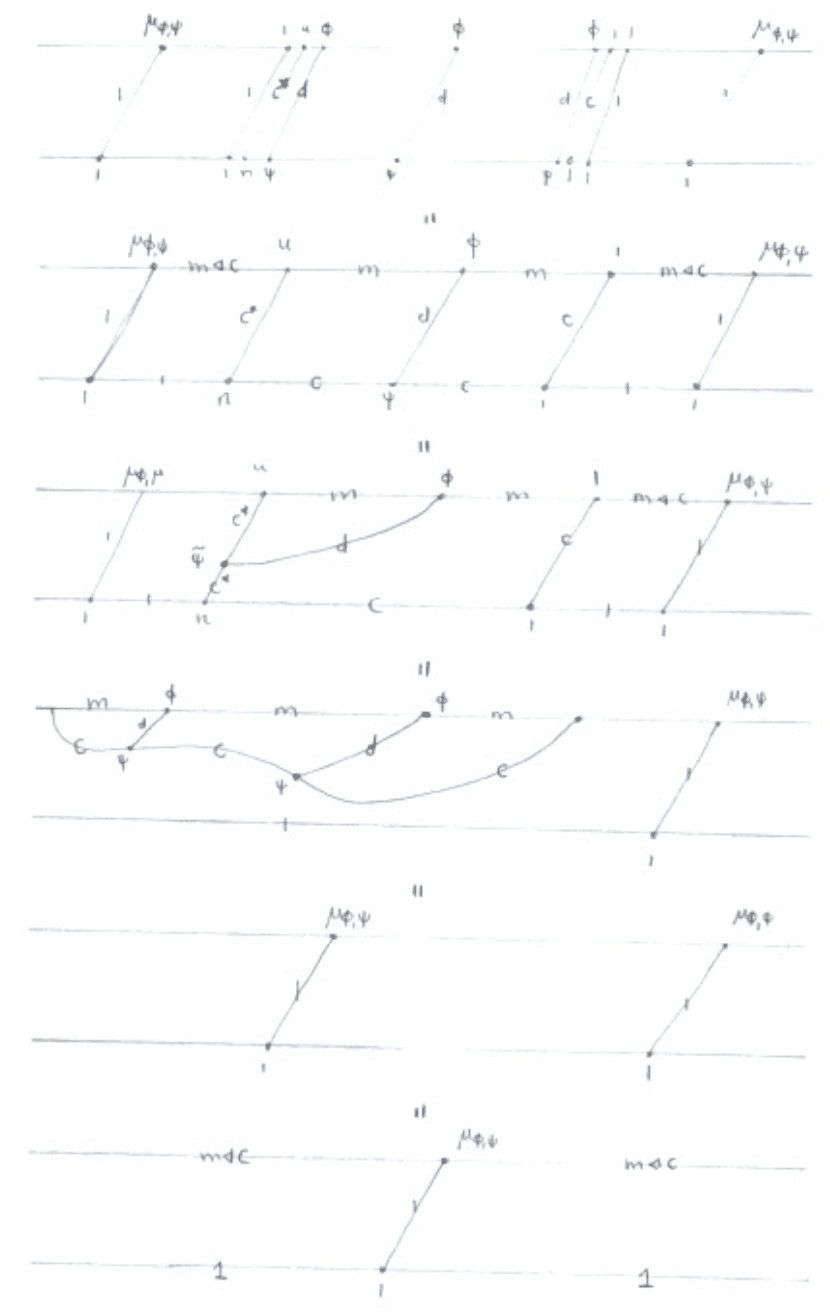
\includegraphics[width=8cm]{4}
  %   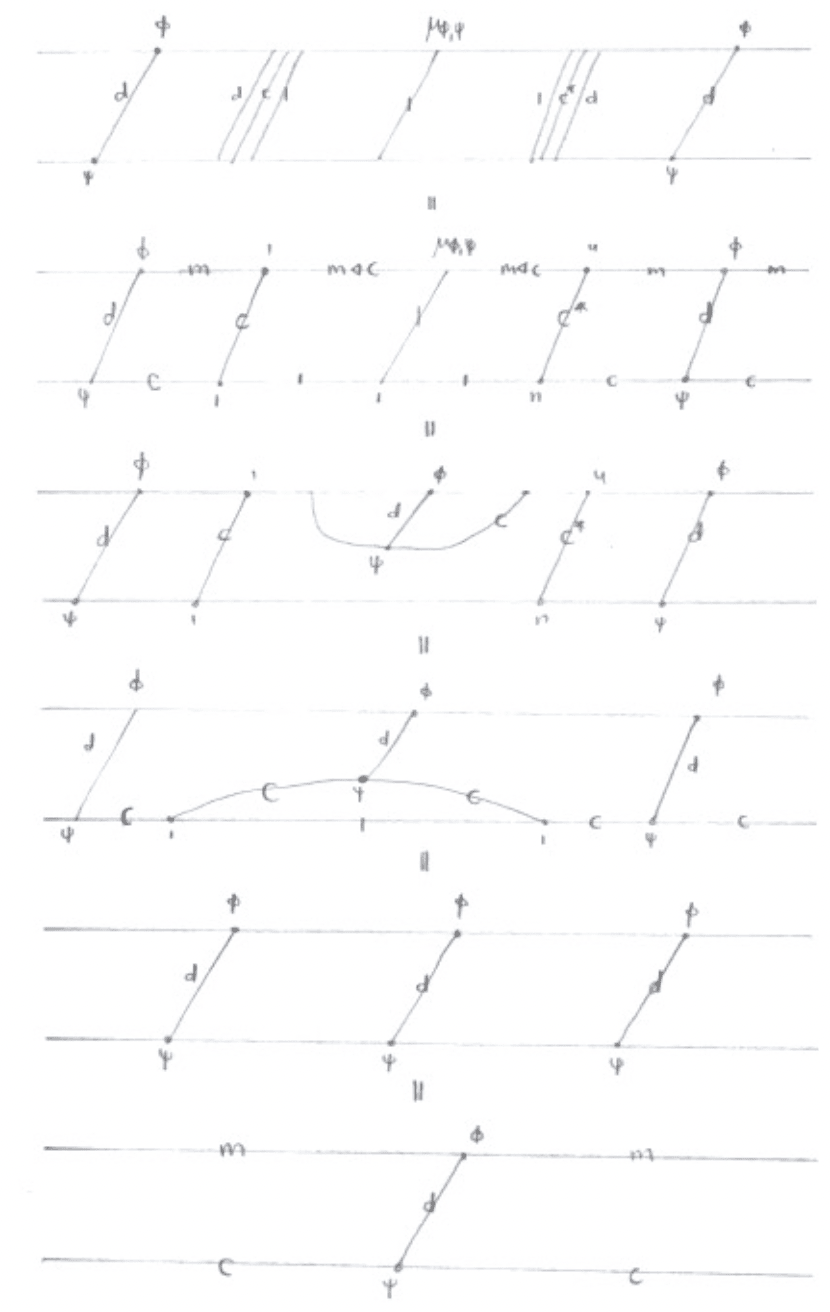
\includegraphics[width=8cm]{5}
  % \end{center}

  \begin{center}
    \includesvg[width=18cm]{drawing-4}
  \end{center}
\end{proof}

\noindent For computation purpose (cf. sec \ref{section/applications}), one
may find the following basis theorem useful.

% TODO I think this is the only place we need semisimplicity and finiteness?
% We many have to fix the definition of skein category as well (it's currently
% defined on simple ones and extend by direct sums), if we are to remove the
% assumptions. // EDIT: Actually no, ss and finiteness makes Deligne products
% easier to handle.
\begin{proposition} (Basis Theorem) \label{proposition/basis-theorem}

  \noindent Let $C$ be a finite, semisimple tensor category, and
  $M_{C}, _{C}N$ be finite, semisimple module categories over $C$. \quad Thus
  the vector spaces $Hom_{M}(m, m' \lhd c), Hom_{N}(c \rhd n, n')$ have finite bases
  $\beta(m, m' \lhd c), \beta(c \rhd n, n')$ respectively. \quad Then the hom space
  $Hom_{p.sk(M,C,N)}(m \boxtimes n, m' \boxtimes n')$ has a linear basis
  \[
    \bigsqcup_{c \in Irr(C)} \beta(m, m' \lhd c) \times \beta(c \rhd n, n').
  \]
\end{proposition}
\begin{proof}
  This follows immediately from the reductions given in \ref{remark/hom-space-reduction}.
\end{proof}
